%%%%%%%%%%%%%%%%%%%%%%%%%%%%%%%%%%%%%%%%%%%%%%%%%%%%%%%%%%%%%%%
%
% Time representation
%
%%%%%%%%%%%%%%%%%%%%%%%%%%%%%%%%%%%%%%%%%%%%%%%%%%%%%%%%%%%%%%%%

This section is devoted to specify the representation of time within the framework of the possibility theory. First of all, the specification for a single ill-known temporal point shall be explained. Then, the formal specification and the related constraints are given for an ill-known valid-time interval.

\subsection{\label{subsec:ill-known-point-rep}Ill-known time point}
An ill-known time point $X$ is a precise time point that for some reason, it is not fully specified. Note that $X$ has only one possible value but that value is unspecified.

\begin{definition}
\label{def:ill-known-time-point}
\emph{Ill-known time point}\\
Consider a time domain $\T$, uncertainty about the values of the ill-known time point $X$ is given by the possibility distribution $\pi_X$:
\begin{equation}
\label{eq:ill-known-time-point}
\Pi(X) = \pi_X(t) \in \left[0,1\right] , t \in \T
\end{equation}
\end{definition}

\begin{definition}
\label{def:ill-known-domain}
\emph{Domain for an ill-known time point}\\
Consider $\Pow(\T)$ the set of all the possibility distributions over $\T$, and the three fuzzy constants \emph{UNKNOWN} $=\left\lbrace 1/t, t \in \T \right\rbrace$, \emph{UNDEFINED} $=\left\lbrace 0/t, t \in \T \right\rbrace$ and \emph{NULL} $=\lbrace 1/$ \emph{UNKNOWN}, $1/$ \emph{UNDEFINED} $\rbrace$. The domain for an ill-known time point $X$ is given by: 
\begin{align}
\label{eq:ill-known-domain}
\Dom (X) =  \lbrace \Pow(\T) & \cup \mbox{\emph{UNKNOWN}} \\
\nonumber
&\cup \mbox{\emph{UNDEFINED}} \\
\nonumber
&\cup \mbox{\emph{NULL}} \rbrace
%
\end{align}
\end{definition}

It is also possible to specify an ill-known time point by just a set of ill-known constraints plus 



\subsubsection{\label{subsubsec:ill-known-time-datatypes}Datatypes}
The datatypes for an ill-known time point $X$ are shown in Table \ref{tbl:time-point-types}.
\vglue13pt
%\begin{table}[htbp]
\tcap{Data types for a time point}
\centerline{\small DATA TYPES}
\vglue-6pt
\centerline{\small\baselineskip=13pt
\begin{tabular}{c p{2cm} p{2cm}}\\
\hline
1 & A single time point &  $1/x, x \in \T$\\
2 & A possibility distribution in the numeric domain & A fuzzy number or a fuzzy interval.\\
3 & An unknown value & \textbf{UNKNOWN}$= \lbrace1/t, t \in \T \rbrace$\\
4 & An undefined value & \textbf{UNDEFINED}$= \lbrace 0/t, t \in \T \rbrace$\\
5 & A null value & \textbf{NULL} $=\lbrace 1/$Unknown, 1/Undefined $\rbrace$\\
\hline\\
\end{tabular}
\label{tbl:time-point-types}
}

%Example of different uses of the ill-known time value.
\begin{example}
Consider a historical database with data from diplomatic documents. The following fields are stored: the digital identifier \emph{ID} which is the primary key  and the stimated time when the document was sent (field \emph{Date}). Table \ref{tbl:sample-time-point} contains some example data from this database. 
\end{example}

\vglue13pt
%\begin{table}[htbp]
\tcap{Sample of the historical database}
%\centerline{\small DATA TYPES}
\vglue-6pt
\centerline{\small\baselineskip=13pt
\begin{tabular}{c c}\\
\textbf{ID} & Date\\
\hline
23454 & Unknown \\ 
34563 & 11/12/1204 \\
12211 & $\left[7/2/1204,30,30\right]$ \\
23455 & $\left[10,10/6/1204,20/6/1204,15 \right]$ \\
\hline\\
\end{tabular}
\label{tbl:sample-time-point}
} 
 
In that database, for the document with ID=23454, all the dates in the domain are equally possible. Nevertheless, the document 34563 was sent in the crisp (exact) date 11/12/1204. The time for documents 12211 and 23455 are specified with several possibility distributions. The first one is also known as a fuzzy number whereas the second one is also known as a fuzzy interval.
\textcolor{red}{References to the preliminaries}.
 
%\end{example}
 
 


\subsection{\label{subsec:ill-known-interval}Ill-known time interval}


\begin{definition}
\emph{Ill-known time interval}\\
An ill-known time interval denoted by $\left[X, Y\right]$ is a precise time interval that for some reason, its boudaries are not precissely known. The ill-known interval is defined by two ill-known points, namely $X$,$Y$.
In order to know if all the points in the crisp time interval $I=\left[a, b\right]$ are within the boudaries of the ill-known time interval $\left[X, Y\right]$ we define the following two ill-known constraints $C_{1}, C_{2}$ 
\begin{eqnarray}
C_1\stackrel{\triangle}{=}\left(\geq,X\right) \wedge \\
C_2\stackrel{\triangle}{=}\left(\leq,Y\right)
\end{eqnarray}
Note that the boolean operator applied to the constraints is $\bool=\wedge$.
This means that we want to know if all the points in the interval $I$ are greater or equal to $X$ and, at the same time, smaller or equal to $Y$.
\end{definition}

%% equations for the poss and nec!!
The simplified equations for the possibility and the necessity measures are~\cite{Pons2011}:
\begin{eqnarray}
\label{eq:interval-pos}
\Pos\left(\lambda([a,b])\right)&=&\\
\nonumber
\min\bigg(\sup_{a\leq w}\pi_{X}(w),\sup_{b\geq w}\pi_{Y}(w)\bigg)\\
\label{eq:interval-nec}
\Nec\left(\lambda([a,b])\right)&=&\\
\nonumber
\min\bigg(\inf_{a>w}1-\pi_{X}(w),\inf_{b<w}1-\pi_{Y}(w)\bigg).
\end{eqnarray}




\subsubsection{\label{subsubsec:open-interval}Open ill-known time intervals}
Quite often, the user may want to specify time intervals with open boudaries in one or both endpoints. Consider an ill-known time interval $\left[X, Y\right]$. Then it is possible to distinguish between the following two types of open intervals:
\begin{enumerate}
\item
\emph{Completely unknown time interval}: Both starting and ending points are unknown, therefore the hole interval is specified by the \emph{UNKNOWN} constant. Due to the representation, both endpoints, say $X$ and $Y$ are stored. Thus, the interval is stored as $[$ \emph{UNKNOWN}, \emph{UNKNOWN} $]$.
\item
\emph{Semi-open time interval}: Only one of the two ill-known endpoints for the time interval $\left[X, Y\right]$ is unknown. Note that due to the ill-known constraints $C_{1}, C_{2}$ it is not possible a representation like $[$ \emph{UNKNOWN} $, Y]$ or $[X, $ \emph{UNKNOWN} $]$. The solution adopted for this problem is explained in the following paragraph.
\end{enumerate}

\paragraph{Representation of semi-open time intervals}
As mentioned before, the problem resides in the representation of these kind of interval. In order to get a short representation for these intervals, two constants are defined: $FB$ \emph{From the Beggining}: it is only valid for the left value of the interval and $UC$ \emph{Until Changed} (this name is usual in the temporal database community, see ~\cite{Jensen1994}) which is only valid for the right value of the interval. Note that these two constants are aliases for a function that obtains both possibility and necessity measures. 

Because of the ill-known constraints $C_{1}, C_{2}$, a function called \emph{Open} should be defined in order to deal with a proper representation of these intervals:

\begin{definition}
\label{def:open-func}
$Open(C)$\\
The function $\Open(C)$ provides both possibility and necessity measures for all the points in the open part of a semi-open ill-known time interval.
The parameter $C$ is an ill-known constraint $C\stackrel{\triangle}{=}\left(R,T\right)$ as defined in equation \eqref{rand} and in~\cite{Pons2011}.
The possibility and necessity measures are defined by:
\begin{eqnarray}
\label{eq:open-pos-nec}
\Pos\left(\Open(C)\right) &=& \Big(\sup_{r\in\T \Rp\  w}\pi_{T}(w)\Big)\\
\Nec\left(\Open(C)\right) &=& \Big(\inf_{r\in\T \Rn\  w}1-\pi_{T}(w)\Big)
\end{eqnarray}
Where the values for the binary relations $\Rp$ and $\Rn$ are shown in Table \ref{tbl:open-pos-nec-rels}.
\end{definition} 

\vglue13pt
%\begin{table}[htbp]
\tcap{Relations for the $\Open(C)$ function.}
\centerline{\small Relations}
\vglue-6pt
\centerline{\small\baselineskip=13pt
\begin{tabular}{c c c}\\
\hline
$R$ & $\Rp$ & $\Rn$\\ \hline
$<$ & $>$ & $\leq$ \\
$\leq$ & $\geq$ & $<$ \\
$>$ & $<$ & $\geq$ \\
$\geq$ & $\leq$ & $>$ \\
\hline\\
\end{tabular}
\label{tbl:open-pos-nec-rels}
}

As explained before, the constants $\FB$ and $\UC$ are aliases for the function $\Open$ with the following parameters:
\begin{eqnarray}
\FB &=& \Open(C_2)\\
\UC &=& \Open(C_1)
\end{eqnarray}


\begin{example}
Consider an ill-known time interval given by $\left[\FB, Y \right]$. Consider also that in this case, $Y= \left[15/10/2012,3,4 \right] $. Figure \ref{fig:example-open-time-interval} shows the representation for $Y$. The user wants to obtain the possibility and the necessity measures for the $\FB$ part of the interval are:
\end{example}

\begin{eqnarray}
\nonumber
\FB = \Open(C_2) \mbox{ with } C_2\stackrel{\triangle}{=}\left(\leq,Y\right)\\
\nonumber
\Pos\left(\Open(C)\right) = \Big(\sup_{r\in\T \geq\  w}\pi_{Y}(w)\Big)\\
\nonumber
\Nec\left(\Open(C)\right) = \Big(\inf_{r\in\T <\  w}1-\pi_{Y}(w)\Big)
\end{eqnarray}


\vspace*{13pt}
\begin{center}
{
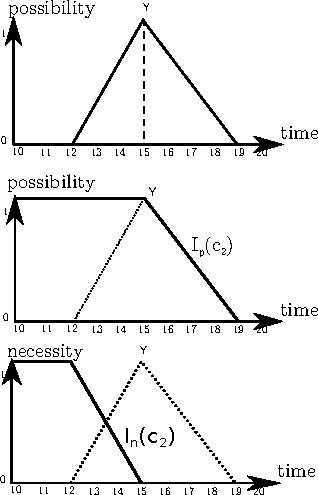
\includegraphics[scale=1]{./graphs/open-time-interval.pdf}
\label{fig:example-open-time-interval}
}
\end{center}
%\centerline{ 
\psfig{file=./graphs/Y-time-point.eps}}
\vspace*{10pt}
\fcaption{Possibility distribution for $Y$, and possibility and necessity measures for the open ill-known point, $X$}
\vspace*{13pt}

\subsubsection{\label{subsubsec:ill-known-time-interval-datatypes}Datatypes}
In order to represent properly an ill-known time interval in a database, some datatypes are needed. Because of the ill-known constraints, not all the combinations of datatypes for each ill-known time point (see Table \ref{tbl:time-point-types}) are allowed. Table \ref{tbl:time-interval-types} shows all the possible combinations for the datatypes for an ill-known time interval denoted by $\left[X, Y\right]$.

\vglue13pt
%\begin{table}[htbp]
\tcap{Data types for an ill-known time interval $\left[X, Y\right]$.}
\centerline{\small DATA TYPES}
\vglue-6pt
\centerline{\small\baselineskip=13pt
\begin{tabular}{c c p{2cm}}\\
\hline
$X$  & $Y$  & Description\\
\hline
$\lbrace1,2 \rbrace$ & $\lbrace1,2 \rbrace$ &  an ill-known time interval.\\
3 & 3 & An unknown time interval. \\
$\FB$ & $\lbrace1,2 \rbrace$ & a left-open time interval.\\
$\lbrace1,2 \rbrace$ & $\UC$ & a right-open time interval.\\
\hline\\
\end{tabular}
\label{tbl:time-interval-types}
}



%\subsection{\label{subsec:time-interval-constraint}Ill-known valid time-interval}
%The representation of a possibilistic valid-time interval is given by two ill-known points: $\left[S,E \right]$ the starting and ending points respectively.  
%
%
%A valid temporal interval $\left[S,E\right]$ in the system is a combination for the values of $S$,$E$. Note that the only allowed combination of types is shown in table \ref{tbl:valid-time-interval}. 
